\documentclass[runningheads]{llncs}
\usepackage[]{algorithm2e}
\usepackage[]{algorithmic}
\usepackage{bm,hyperref,booktabs,tikz,pgf,pgfplots,amsmath}
\usetikzlibrary{arrows,automata,circuits}
%\pgfplotsset{compat=1.13}
%\usepackage{pgfkeys}
%\usepackage{graphicx}
%xcolor} 
%amsmath} 
%amstext} 
%amssymb} 
%amsfonts} 
%\usepackage{mathptmx} 
%\usepackage[scaled=.90]{helvet} 
%\usepackage{courier} 
%\usepackage{textcomp} 
%\usepackage{array}
%\usepackage{varwidth}
%\usepackage[american]{babel}
%usepackage{mathtools} % fixes and extends amsmath
%mathtoolsset{mathic}
%\allowdisplaybreaks
%\usepackage{mathptmx}
%\usepackage{tabu}
%%\usepackage{breqn}
%\usepackage{algorithm,algorithmic,bm}
% If you use the hyperref package, please uncomment the following line
% to display URLs in blue roman font according to Springer's eBook style:
%\renewcommand\UrlFont{\color{blue}\rmfamily}
%% Suggested packages, as needed:
%\usepackage{booktabs} % commands to create good-looking tables
%\usepackage{tikz} % nice language for creating drawings and diagrams - required for 
%drawing custom shapes
%\usetikzlibrary{%
%	arrows,%
%	calc,%
%	fit,%
%	patterns,%
%	plotmarks,%
%	shapes.geometric,%
%	shapes.arrows,%
%	shapes.callouts,%
	% shapes.multipart,%
	% shapes.gates.logic.US,%
	% shapes.gates.logic.IEC,%
	% er,%
	% automata,%
%	topaths,%
%	trees,%
%	matrix,%
%	% calendar,%
%	folding,%
%	fadings,%
%	positioning,%
%	scopes,%
%	decorations.fractals,%
%	decorations.shapes,%
%	decorations.text,%
%	decorations.pathmorphing,%
%	decorations.pathreplacing,%
%	decorations.footprints,%
%	decorations.markings,%
%	shadows}
%\usepackage{trace-pgfkeys}
\begin{document}
\title{Approximating Information-Theoretic Scores\\for Computer Adaptive Tests\\in Bayesian and Credal Networks}
%%\thanks{Supported by organization x.}}
%\titlerunning{Abbreviated paper title}
\author{Alessandro Antonucci \and
Francesca Mangili \and\\
Claudio Bonesana \and
Giorgia Adorni}
%\authorrunning{F. Author et al.}
\institute{Istituto Dalle Molle di Studi sull'Intelligenza Artificiale, Lugano, Switzerland\\
\email{\{alessandro,francesca,claudio.bonesana,giorgia.adorni\}@idsia.ch}}
\maketitle
\begin{abstract}
A test is adaptive when the sequence and the number of questions is tuned on the basis of the estimated skills of the test taker. Graphical models such as Bayesian networks allow to model the uncertainty about the questions and the skills in an highly interpretable fashion, especially when coping with multiple skills. Yet, the quantification of the uncertainty in the question/skill relations can be better quantified by interval-valued probabilistic values in the model. This might make inference considerably harder in the underlying model, this being especially the case for the information theoretic quantities generally used as a score to drive the adaptation process.
Here we present an alternative score based on the mode of the posterior probabilities of the model. We show how this makes considerably simpler the evaluation of the score in the credal case. Numerical tests are promising, we show how the performance are similar in the Bayesian network case, while xxx.
%considered. 
%We propose an alternative 
%We present.
%with xxx. Interval valued quantification
%We suggest the use of credal networks, a generalization of Bayesian networks based on sets of probability mass functions, to implement adaptive tests exploiting the knowledge of the test developer instead of training on databases of answers. Compared to Bayesian networks, these models might offer higher expressiveness and hence a more reliable modeling of the qualitative expert knowledge. The counterpart is a less straightforward identification of the 
%information-theoretic measure controlling the question-selection and the test-stopping criteria. We elaborate on these issues and propose a sound and computationally feasible procedure. Validation against a Bayesian-network approach on a benchmark about German language proficiency assessments suggests that credal networks can be reliable in assessing the student level and  effective in reducing the number of questions required to do it.
%150-200 words - 12 pages
\keywords{First keyword  \and Second keyword \and Another keyword.}
\end{abstract}


\section{A Toy Example}
As a first, demonstrative, example of our ideas consider a model characterized by a single (Boolean) Skill $S$ and a set of questions $\bm{Q}$ picked from a set of templates. Let us first focus on a Bayesian, i.e., precise, case. The prior specification $P(S)$ is achieve by a single parameter $p \in [0,1]$ such that $P(S=1)=p$. For a generic question $Q$, which is also assumed to be Boolean, a complete specification of the CPT $P(Q|S)$ is obtained by the two parameters $p_0,p_1\in [0,1]$ where $P(Q=1|S=0)=p_0$ and $P(Q=1|S=1)=p_1$. In other wrods $p_0$ denote the probability of providing a right answer to the question for a student who does not have the considered skill and $p_1$ for a student who have that skill. An obvious constraint is $p_1>p_0$, i.e., having the skill makes your probability of providing a right answer higher. The inequality should be strict, otherwise the two probabilities are equal, and this means that the answer is irrelevant for the skill. Although parameters $p_1$ and $p_0$ already give a complete parametrization, we perform the linear transformation
$\lambda:=1-\frac{1}{2}(p_0+p_1)$ and $\delta=(p_1-p_0)$. The first quantity is the arithmetic average of giving a wrong answer and we might indent it as the \emph{level} of the question, this mining that the higher is $\lambda$ the more unlikely is to receive a correct answer is the students have the same probability of having and not having the skill. Regarding $\delta$ we might intend it as the (average) discriminative power of a question.
Note that the inverse relations give $p_1=1-\lambda+\frac{\delta}{2}$
and $p_0=1-\lambda-\frac{\delta}{2}$. Where constraint $p_1>p_0$ is just $\delta>0$ and any other value in $[0,1]$ for both parameters is valid.


In our toy example, we consider nine possible templates, made of triads of templates with the same $\delta$ and same $\lambda$. The reference values $[0.4,0.5,0.6]$ are used.





\section{Testing Algorithms}
The typical goal of a test or exam is to evaluate the knowledge level of a student or examinee $\sigma$ on the basis of her answers to a number of questions or exercises. Let $\bm{Q}$ denote a repository of questions available to the instructor. The order and the number of questions from $\bm{Q}$ asked to $\sigma$ might not be fixed. We call \emph{testing algorithm} (TA) a procedure taking care of the selection of the sequence of questions asked to the student and able to decide when the test should stop. A standard TA pseudocode is in Algorithm \ref{alg:ta}, where $\bm{e}$ denotes the array of the answers collected from the student $\sigma$.



\begin{algorithm}[H]
    \SetAlgoLined
    \KwResult{Write here the result }
    initialization\;
    \While{While condition}{
        instructions\;
        \eIf{condition}{
            instructions1\;
            instructions2\;
        }{
            instructions3\;
        }
    }
    \caption{How to write algorithms}
\end{algorithm}

\begin{algorithm}[htp]
    \begin{algorithmic}[1]
    \STATE $\bm{e}=\emptyset$
        \WHILE{ {\bf not} $\tt{Stopping}(\bm{e})$}
        \STATE $Q^* \gets \tt{PickQuestion}(\bm{Q},\bm{e})$
        \STATE $q^* \gets {\tt{Answer}}(Q^*,\sigma)$
        \STATE $\bm{e} \gets \bm{e} \cup \{ Q^*=q^* \}$
        \STATE $\bm{Q} \gets \bm{Q} \setminus \{ Q^*\}$
        \ENDWHILE
        \STATE {\bf return} $\tt{Evaluate}(\bm{e})$
    \end{algorithmic}\label{alg:ta}
\caption{Testing algorithm. Student profile $\sigma$ and question repository $\bm{Q}$ are inputs.}
\end{algorithm}


The Boolean function ${\tt Stopping}$ decides whether or not the test should end, this choice being possibly based on the previous answers as collected in $\bm{e}$. Trivial examples of such stopping rules might be based on the number of questions asked to the student (${\tt Stopping}(\bm{e})=1$ if and only if $|\bm{e}|>n$) or on the number of correct answers provided that a maximum number of questions is not exceeded. Function ${\tt PickQuestion}$ is instead in charge of deciding which question should be asked to the student from the repository $\bm{Q}$. A TA is called \emph{adaptive} when this function is based on the previous answers $\bm{e}$. Trivial non-adaptive strategies might consist in randomly picking an element of $\bm{Q}$ or following a fixed order. Function ${\tt Answer}$ is simply collecting (or simulating) the answer of the student $\sigma$ to a particular question $Q$. In our assumptions, this answer is not affected by the previous answers to other questions.\footnote{Generalized setups where the quality of the student answer is affected by the previous answers will be discussed at the end of the paper. This might include a \emph{fatigue} model negatively affecting the quality of the answers when many questions have been already answered as well as the presence of \emph{revealing} questions that might improve the quality of other answers.} 

Finally, the ${\tt Evaluate}$ function decides the overall judgement for the test (e.g., a numerical grade or a pass/fail Boolean) on the basis of all the answers collected after the test termination. Trivial examples of such function are the percentage of correct answers or a Boolean that is true when a sufficient percentage of correct answers has been provided. Note also that in our assumptions the TA is \emph{exchangeable}, i.e., the stopping rule, the question finder and the evaluation function are invariant with respect to permutations of $\bm{e}$. In other words, the would pick the same next question and the same evaluation for two students who provided the same list of answers in two different orders and similarly would decide to stop or not to stop in the same way. 

The typical goal of a TA is to achieve a reliable evaluation of the student $\sigma$. As each answer is assumed to improve such quality, asking all the questions, no matter their order because of the exchangeability assumption, would be an obvious choice. Yet, asking all the questions in the repository might be impractical (e.g., because of time limitations) in some cases or just provide an unnecessary burden to the students. The goal of a good TA is therefore to trade off the accuracy of the evaluation and the number of questions.\footnote{In some generalized setups, other elements such as the \emph{serendipity} to avoid boring sequences of questions might be also considered.}

Item response theory is a popular *** Something about IRT here ***. Most of these approaches are based an a unidimensional representation of the student knowledge level. Proposals to cope with multidimensional IRTs have been considered, but this results critical when coping with dependencies between them. For this reason probabilistic modelling can be considered. This is the topic of the next section.

\section{Bayesian Adaptive Testing Algorithms}
In the setup of algorithm.

Let us introduce the discussion by means of a simple example modelling the knowledge level of a student in a particular domain. In order to evaluate such level a number of questions can be asked to the student. We describe the knowledge level (or skill) of the student by means of a single variable $S$. We assume $S$ to be a discrete, ordinal, variable, whose $m$ states $\mathcal{S}:=(s^{(0)},\ldots,s^{(m-1)})$ can be intended as increasing knowledge levels in that domain. Regarding the questions, we initially describe them as Boolean variables, whose true state correspond to a correct answer to the question, while no distinctions between the possible wrong answers are considered.\footnote{Dedicated discussion about abstention.} Let $Q$ with $\mathcal{Q}:=(q,\overline{q})$ denote a generic question we ask to the student. A repository of $n$ questions $\bm{Q}$ is assumed to be available. A \emph{testing} algorithm is a procedure deciding which question and how many questions from $\bm{Q}$ should be asked to the student, on the basis of her previous answers. Algorithm X provides an abstract description of xxx.


	%
	%
	\section{Brainstorming}
	
	\subsection{Linear Programs for Credal Mode}
	
	Given the Boolean question $Q$ and the Boolean skill $S$, we use the score:
	
	\begin{equation}
		\sigma_Q := \max_{P\in K} \bigl[ 
		\max \{ P(S=0,Q=0) , P(S=1,Q=0) \}  + \max \{ P(S=0,Q=1),P(S=1,Q=1)\}
		\bigr]
	\end{equation}
	
	\begin{theorem}
		\begin{equation}
			\max_{x}  \max \{ f(x) , g(x) \}  
			=
			\max \{ \max_{x'} f(x') , \max_{x''} g(x'') \} 
		\end{equation}
		Let 
		$$y^{*}:=\max_x \max\{f(x),g(x)\}$$
		$$y^{**}:= \max \{ \max_{x'} f(x') , \max_{x''} g(x'') \}$$
		Say for instance that $y^{**}=max_x f(x)$ and let $x^{**}:=\arg\max_x f(x)$. Thus:
		$$f(x^{**})\geq \max_{x'} g(x) \geq g(x^{**})$$ 
		
		Let $x^{*}:= \arg\max_x \max\{f(x),g(x)\}$. 
		It cannot be $y^{*}:=g(x^{*})$ as this would imply $g(x^{*}) \geq f(x^{*})$ 
		
		
		%Assume ad absurdum $y^{*}\neq y^{**}$.
		
		
		If $y^{*}:=f(x^{*})$ we should have $y^{*}=y^{**}$.
		Vice versa, 
		
		or
		%$y^{*}:=g(x^{*})$. In the first case 
	\end{theorem}
	
	
	
	\subsection*{Pseudocode}
	Let us first specify the inputs:
	\begin{itemize}
		\item Let $\bm{S}:=(S_1,\ldots,S_N)$ denote the set of skills in the model. We 
		describe a \emph{student} as a joint observation $\bm{s}$ of the skills.
		\item Let $M$ denote the network \emph{skeleton}, i.e., the model over the skills only
		\item A question $Q$ is a binary variables with states right and wrong
		\item Each question depends on a single skill only, let $\mathrm{Pa}(Q)$ denote this 
		skill
		\item Let $\tau(S)$ denote the number of \emph{templates} for the CPT of a question 
		associated with $S$, $\{P(Q|S)\}_{t=1}^{\tau(S)}$ 
		\item Let $n_q$ be the maximum number of questions we might ask for each skill
	\end{itemize}
	The algorithm works as follows.
	\begin{enumerate}
		\item For eachLet $\bm{S}:=(S_1,\ldots,S_N)$ denote the set of skills in the model
		\item Let $M$ denote the network \emph{skeleton}, i.e., the model over the skills only
		\item A question $Q$ is a binary variables with states right and wrong
		\item Each question depends on a single skill only, let $\mathrm{Pa}(Q)$ denote this 
		skill
		\item Let $\tau(S)$ denote the number of \emph{templates} for the CPT of a question 
		associated with $S$, $\{P(Q|S)\}_{t=1}^{\tau(S)}$ 
		\item Let $n_q$ be the maximum number of questions we might ask for each skill
	\end{enumerate}
	
%	\begin{algorithm}[htp!]
%		\caption{Single skill, precise model\\
%			a model (BN, skeleton) $M$ over the skills only
%			\\a dataset of $n$ students $\{s^i\}_{i=1}^n$,\\a dataset of $m$ questions 
%			$\mathcal{Q}:=\{Q^j\}_{j=1}^m$,\\
%			the CPTs of the questions in $\mathcal{Q}$, i.e., $\{P(Q^j|S)\}_{j=1}^m$\\
%			the student answer models $\{\tilde{P}(Q^j|S)\}$\\
%			an entropy threshold $h^*$,\\
%			a score function for questions $\gamma$
%			\label{alg:simple}}
%		\begin{algorithmic}[1]
%			\FOR {$i\gets\{1,\ldots,n\}$}
%			\STATE $(M',\mathcal{Q}',\mathcal{Q}'',\bm{e}) \gets 
%			(M,\mathcal{Q},\emptyset,\emptyset)$
%			\WHILE{ $h > h^* \mathrm{\bf and}\, \mathcal{Q}' \neq \mathcal{Q}$}
%			\STATE $Q^* \gets \arg\max_{Q \in \mathcal{Q}'}\gamma(M',Q,\bm{e})$
%			\STATE{$\mathcal{Q}'\gets \mathcal{Q}' \setminus \{ Q^*\}$}
%			\STATE{$\mathcal{Q}''\gets \mathcal{Q}'' \cup \{ Q^*\}$}
%			\STATE{$q^* \gets \mathrm{sampling} \sim \tilde{P}(Q^*|s^i)$}
%			\STATE $M' \gets \mathrm{addChild}(M',Q,S,P(Q|S))$
%			\STATE $\bm{e} \gets \bm{e} \cup \{ Q^*=q^* \}$
%			\STATE $h \gets H[P_{M'}(S|\bm{e})]$
%			\ENDWHILE
%			\STATE $\sigma_i \gets \arg\max_{s\in\mathcal{S}} P_{M'}(s|\bm{e})$
%			\ENDFOR
%			\STATE {\bf return} $(\sigma_1,\ldots,\sigma_n)$
%		\end{algorithmic}
%	\end{algorithm}
	Three possible scores:
	\begin{eqnarray}
		\gamma(Q,\bm{e}) := -H[S|Q,\bm{e}] = -\sum_q P(q) \cdot H[S|\bm{e},q]&&\\
		\gamma'(Q,\bm{e}) :=  -\sum_q P(q) \cdot \max_{s\in\mathcal{S}}  P[s|\bm{e},q]&&\\
		\gamma''(Q,\bm{e}) :=  |P(Q=1|\bm{e})-0.5|&&
	\end{eqnarray}
	
	\textcolor{red}{Maybe, instead of (3) I would use a known measure of qualitative 
	variation (\url{https://en.wikipedia.org/wiki/Qualitative_variation}) which extend easily to 
	non binary answers, e.g., the variation ratio ($1-\max_q(P(q))$) or the M1 Gibb's index 
	also known as coefficient of unalikeability and somehow related to the variance (it is 
	the variance in the binary case): $M1 = 1-\sum_q P(q)^2$, or even the entropy, which is 
	not so difficult to compute for $P(Q)$. They are all equivalent in the binary case, as 
	they are all monotonic function of $\max_q(P(q))$ only. }
	
	
%	\begin{algorithm}[htp!]
%		\caption{Single skill, credal model\\a dataset of $n$ students $\{s^i\}_{i=1}^n$,\\a 
%		dataset of $m$ questions $\mathcal{Q}:=\{Q^j\}_{j=1}^m$,\\
%			the credal CPTs of the questions in $\mathcal{Q}$, i.e., 
%			$\{\overline{P}(Q^j|S)\}_{j=1}^m$\\
%			an upper entropy threshold $\overline{h}^*$,\\
%			a score function for questions $\sigma$
%			\label{alg:simple2}}
%		\begin{algorithmic}[1]
%			\FOR {$i\gets\{1,\ldots,n\}$}
%			\STATE $(\mathcal{Q}',\mathcal{Q}'',\bm{e}) \gets 
%			(\mathcal{Q},\emptyset,\emptyset)$
%			\WHILE{ $h > h^* \mathrm{\bf and}\, \mathcal{Q}' \neq \mathcal{Q}$}
%			\STATE $Q^* \gets \arg\max_{Q \in \mathcal{Q}'}\gamma(Q,\bm{e})$
%			\STATE{$\mathcal{Q}'\gets \mathcal{Q}' \setminus \{ Q^*\}$}
%			\STATE{$\mathcal{Q}''\gets \mathcal{Q}'' \cup \{ Q^*\}$}
%			\STATE{$q^* \gets \mathrm{sampling} \sim P(Q^*|s^i)$}
%			\STATE $\mathrm{addChild}(Q,S,P(Q|S))$
%			\STATE $\bm{e} \gets \bm{e} \cup \{ Q^*=q^* \}$
%			\STATE $h \gets H[P(S|\bm{e})]$
%			\ENDWHILE
%			\STATE $\sigma_i \gets \arg\max_{s\in\mathcal{S}} P(s|\bm{e})$
%			\ENDFOR
%			\STATE {\bf return} $(\sigma_1,\ldots,\sigma_n)$
%		\end{algorithmic}
%	\end{algorithm}
	Three possible scores:
	\begin{eqnarray}
		\gamma(Q,\bm{e}) := -H[S|Q,\bm{e}] = -\sum_q P(q) \cdot H[S|\bm{e},q]&&\\
		\gamma'(Q,\bm{e}) :=  -\sum_q P(q) \cdot \max_{s\in\mathcal{S}}  P[s|\bm{e},q]&&\\
		\gamma''(Q,\bm{e}) :=  |P(Q=1|\bm{e})-0.5|&&
	\end{eqnarray}
	
	
	
	
%	\begin{algorithm}[htp!]
%		\caption{Given a dataset of student profiles $\bm{S}$\label{alg:simple3}}
%		\begin{algorithmic}[1]
%			\FOR {$s\in\bm{S}$}
%			\WHILE{ $h > h^*$}
%			\STATE $Q^* \gets \mathrm{FindBestQuestion}(\bm{Q}$)
%			\STATE $q^* \gets \mathrm{SimulateAnswer}(\sigma)$
%			\STATE $\bm{e} \gets \bm{e} \cup \{ Q^*=q^* \}$
%			\STATE $h \gets H[P(S|\bm{e}]$
%			\ENDWHILE
%			\ENDFOR
%			\STATE {\bf return} $\arg\max P(s|\bm{e})$
%		\end{algorithmic}
%	\end{algorithm}
	
	
	
	
	
	\subsection*{Formulae}
	Let us define the functions, all defined for $x\in [0,1]$, apart from $f$ defines for each 
	$x\geq 0$:
	\begin{eqnarray}
		f(x)&:=& \frac{1}{1+x},\,,\\
		h(x)&:=&-x \cdot \log_2 x - (1-x)  \cdot \log_2 (1-x)\,,\\
		l(x)&:=&\frac{x}{1-x}\,,\\
		m(x)&:=&2 \max\{x,1-x\}\,,\\
		i_\epsilon(x)&:=&\epsilon\log(e^{\frac{2x}{\epsilon}}+e^{\frac{2(1-x)}{\epsilon}})\,,\\
		\tilde{i}_\epsilon(x)&:=&\frac{i_\epsilon(x)-i_\epsilon(0)}{i_\epsilon(\frac{1}{2})-i_\epsilon(0)}\,.
	\end{eqnarray}
	
	Derivatives:
	\begin{eqnarray}
		f'(x)&:=& -\frac{1}{(1+x)^2},\,,\\
		h'(x)&:=&\log_2 \frac{1-x}{x}\,\\
		G(x) &:=& h \circ f(x)\,\\
		G'(x) &:=& h[f(x)] f'(x)=-\frac{\log_2\frac{1-f(x)}{f(x)}}{(1+x)^2}\,\\
		G'(x) &:=& -\frac{\log_2 x}{(1+x)^2}\,\\
		l(x)&:=&\frac{x}{1-x}\,,\\
		m(x)&:=&2 \max\{x,1-x\}\,,\\
		i_\epsilon(x)&:=&\epsilon\log(e^{\frac{2x}{\epsilon}}+e^{\frac{2(1-x)}{\epsilon}})\,,\\
		\tilde{i}_\epsilon(x)&:=&\frac{i_\epsilon(x)-i_\epsilon(0)}{i_\epsilon(\frac{1}{2})-i_\epsilon(0)}\,.
	\end{eqnarray}
	
	
	
	
	A few remarks. Function $f$ is a monotonically decreasing function with values in 
	$[0,1]$. Function $h(x)$ corresponds to the entropy of a mass function over a Boolean 
	variable with a probability equal to $x$. On the extreme points of its domain, we take 
	the limit value, i.e., zero. The function is unimodal and achieve its maximum on  
	$x=\frac{1}{2}$. Function $l$ is the popular \emph{logit} function, it is monotonically 
	increasing function of $x$ and $l(1-x)=l(x)^-1$. Function $m(x)$ is $x$ for $x\geq 
	\frac{1}{2}$ and $1-x$ otherwise. 
	Exactly as $h$, functions $m$ and $\tilde{i}_\epsilon$, for each $\epsilon>0$, have the 
	same (zero) value for $x=0$ and $x=1$, being all unimodal with maximum in 
	$x=\frac{1}{2}$.
	Finally, the popular Gumbel's trick implies:
	\begin{equation}
		\lim_{\epsilon \to 0} i_\epsilon(x)= 
		\lim_{\epsilon \to 0} \tilde{i}_\epsilon(x)
		= m(x)\,.
	\end{equation}
	\subsection*{Another Formula}
	Consider a PMF $P(X)$. Let $x^*:=\arg\max_{x\in\mathcal{X}} P(x)$. Let $\mathcal{P}$ 
	denote the set of all PMFs with the same $p^*:=P(x^*)$. The most entropic PMF in 
	$\mathcal{P}$ is the one with  $P(x)=\frac{1-p^*}{m-1}$ for each $x\neq x^*$ where 
	$m:=|\mathcal{X}|$. While the least entropic is the one with a 
	$x'\in\mathcal{X}\setminus\{x^*\}$ such that $P(x')=1-p^*$ and all the other masses 
	equal to zero. These two bounds on the entropy are therefore:
	\begin{eqnarray}
		\overline{h}&:=& -p^* \log_m p^* - (1-p^*) \log_m \frac{1-p^*}{m-1}\,,\\
		\overline{h}&:=& -p^* \log_m p^* - (1-p^*) \log_m (1-p^*)\,.
	\end{eqnarray}
	This:
	\begin{equation}
		\overline{h}-\underline{h}=(1-p^*) \log_m (m-1)\,,
	\end{equation}
	The maximum gap between the entropies of the PMFs in $\mathcal{P}$ decreases as 
	soon as $p^*$ increases and as soon as the number of states of $X$ decreases, being 
	zero for binary variables.
	
	\subsection*{Toy Example}
	Consider a Boolean skill $S$ with states $s_0$ and $s_1$ and a Boolean 
	question/answer $Q$. Let us shape the model as a BN, $S\to Q$. The prior $P(S)$ is 
	specified by a parameter $p:=P(s_1)$. The question CPT $P(Q|S)$ might be specified 
	instead by two parameters $\pi_1:=P(q_1|s_1)$ and $\pi_0:=P(q_1|s_0)$. The 
	informativeness score we assign two the question is
	\begin{equation}
		\sigma_Q = H[S|Q]:=H[S|q_0]P(q_0)+H[S|q_1]P(q_1)\,.
	\end{equation}
	We have
	\begin{equation}
		P(q_1)=\pi_1 p + \pi_0 (1-p)
	\end{equation}
	while $P(q_0)=1-P(q_1)$ and also
	\begin{equation}
		P(s_1|q_1)=\frac{\pi_1 p}{\pi_1 p + \pi_0 (1-p)}=\frac{1}{1+\frac{\pi_0(1-p)}{\pi_1 p}}
	\end{equation}
	and
	\begin{equation}
		P(s_1|q_0)=\frac{p (1-\pi_1)}{p(1-\pi_1) +  (1-p)(1-\pi_0)} = \frac{1}{1+ \frac{ 
		(1-p)(1-\pi_0)}{p (1-\pi_1)}} 
	\end{equation}
	while $P(S=0|Q=1)$ by normalization. Accordingly:
%	\begin{multline}
%		\sigma_Q(p,\pi_0,\pi_1)=\\
%		h \circ f[\gamma/l(p)] \cdot t +
%		h \circ f[\gamma'/l(p)] \cdot (1-t)\,
%		%\theta(\frac{\pi_0(1-p)}{\pi_1 p}) [\pi_1 p + \pi_0 (1-p)]\\
%		%+ \theta(\frac{ (1-p)(1-\pi_0)}{p (1-\pi_1)}) [1-\pi_1 p + \pi_0 (1-p)]
%	\end{multline}
	where $\gamma = \frac{\pi_0}{\pi_1}$, $\gamma' = \frac{1-\pi_0}{1-\pi_1}$, and $t = \pi_1 
	p + \pi_0 (1-p)$.
	
	{\color{blue}{In other words:
			$\sigma_Q(p,\pi_0,\pi_1):= G(\frac{1-p}{p} \frac{1-\pi_0}{1-\pi_1}) (1-p) + 
			G(\frac{1-p}{p} \frac{\pi_0}{\pi_1}) p$}}
	
	
	
	An alternative score might be achieved by replacing $h$ with $m$, i.e.,
	\begin{equation}
		\sigma_Q' := 
		m \circ f[\gamma/l(p)] \cdot t +
		m \circ f[\gamma'/l(p)] \cdot (1-t)\,
	\end{equation}
	As $f$ is monotone, we can commute $m$ and $f$ *** explain ***, i.e.,
	\begin{equation}
		\sigma_Q' := 
		f \circ m[\gamma/l(p)] \cdot t +
		f \circ m[\gamma'/l(p)] \cdot (1-t)\,
	\end{equation}
	with, as $\gamma>0$. $f \circ m[\gamma/l(p)] = f[\gamma m(l(p))]$
	We can similarly define another score $\sigma_Q''$ based on $\tilde{i}_\epsilon$.
	\subsection*{Explicit maximization}
	$$H[S|Q]\simeq \sigma_Q' = \sum_q P(s^*(q)|q) P(q)$$
	where $s^*(q):=\arg\max_s P(s|q)$. 
	$$\sigma_Q'= \sum_q P(s^*(q),q) = \sum_q P(s^*(q) P(q|s^*(q))$$
	Note that, if $s^*(q)$ is the same for each $q$, the score just corresponds to $P(s^*)$. 
	In other words, the score is flat is each answer gives the same most likely skill level *** 
	reasonable ***. Let us move to an imprecise setting and intend the $s^*$ state as
	$s^*(q):=\arg\max_s \overline{P}(s|q)$. The objective function is a linear combination of 
	$P(s*(q)$ whose coefficient can be optimized independently. Overall, this corresponds 
	to a linear programming task.
	$$\max_s \overline{P}(s,q) = \max_s \max_P P(s) P(q|s) = \max_s \overline{P}(s) 
	\overline{P}(q|s)$$
	
	\subsection*{Francesca's comments}
	
	Comment1: This sentence is not clear to me:  "as $\gamma>0$. $f \circ m[\gamma/l(p)] 
	= f[\gamma m(l(p))]$".\\
	Comment2: How shall we use the Gumbel's trick
	
	
	Comment 3: Below I obtain something that looks different to me, but maybe it is 
	equivalent.  
	
	\begin{equation}
		P(s_1|q_1)=\frac{\pi_1 p}{P(q_1)}
	\end{equation}
	
%	\begin{multline}
%		\sigma_Q(p,\pi_0,\pi_1)=\\
%		m\bigl(\frac{\pi_1 p}{P(q_1)}\bigr) \cdot P(q_1)  +
%		m\bigl(\frac{(1-\pi_1) p}{1-P(q_1)}\bigr) \cdot (1-P(q_1))\,
%	\end{multline}
	
	But, as $P(q_1)\geq 0$, then
%	\begin{multline}
%		m\bigl(\frac{\pi_1 p}{P(q_1)}\bigr) =\\
%		2max\bigl(\frac{\pi_1 p}{P(q_1)},1-\frac{\pi_1 p}{P(q_1)} \bigr) =\\
%		2max\bigl(\frac{\pi_1 p}{P(q_1)},\frac{\pi_0(1- p)}{P(q_1)} \bigr) =\\
%		\frac{2}{P(q_1)}max\bigl(\pi_1 p,\pi_0(1- p)\bigr).\\
%	\end{multline}
	
	Similarly, as $1-P(q_1)\geq 0$, 
%	\begin{multline}
%		m\bigl(\frac{(1-\pi_1) p}{1-P(q_1)}\bigr) =\\
%		\frac{2}{1-P(q_1)}max\bigl((1-\pi_1) p,(1-\pi_0)(1- p)\bigr),\\
%	\end{multline}
	
	so that,
	
%	\begin{multline}
%		\sigma_Q(p,\pi_0,\pi_1)= \\
%		2 max\{\pi_1 p, \pi_0 (1-p)\}+
%		2 max\{(1-\pi_1 )p, (1-\pi_0) (1-p)\}\,
%	\end{multline}
	
	Comment 4: The optimisation in the credal setting shouldn't be the following one?
	
	$$\max_P [\max_s P(s,q=0)+\max_s P(s,q=1)]$$ 
	
	$\P(s,q=0)$ and $P(s,q=1)$ are both functions of $p, \pi_0,$ and $\pi_1$ so I do not 
	think we can split the optimization
	
	$$\max_P \max_s P(s,q=0)+\max_P\max_s P(s,q=1)$$ 
	
	However, it could be a reasonable approximation. Then, we can switch the optimization 
	over $P$ and $s$ because they are both max, and obtain: 
	$$\max_s \overline{P}(s)\overline{P}(q=0|s)+\max_s  \overline{P}(s)\overline{P}(q=1|s)$$.
	
	If instead we are looking for the minimum over P, we cannot switch the optimization 
	over $P$ and $s$:
	$$\min_P \max_s P(s,q) \neq \max_s \min_P P(s,q)$$.
	
	However I think we can split the optimization into 4 quadratic optimizations.
	Let's use the following parametrization:
%	\begin{multline}\label{eq:minimization}
%		\min_{p,\pi_0,\pi_1} \sigma_Q(p,\pi_0,\pi_1) = \\
%		2\min_{p,\pi_0,\pi_1} \bigl( \max\{\pi_1 p, \pi_0 (1-p)\} + \\
%		~~~ \max\{(1-\pi_1 )p, (1-\pi_0) (1-p)\} \bigr) \approx \\
%		2 \bigl( \min_{p,\pi_0,\pi_1}  \max\{\pi_1 p, \pi_0 (1-p)\} + \\
%		~~~ \min_{p,\pi_0,\pi_1} \max\{(1-\pi_1 )p, (1-\pi_0) (1-p)\} \bigr) 
%	\end{multline}
	
	Let's consider the first optimization $\min_{p,\pi_0,\pi_1}  \max\{\pi_1 p, \pi_0 (1-p)\}$. It 
	can be written as
	$$ \min(\tilde{P}(s=0,q),\tilde{P}(s=1,q)) $$ 
	where 

%	\begin{multline}
%		\tilde{P}(s=0,q) = \min_{\pi_1 ,p} \pi_1 p \\
%		\begin{array}{ll}
%			\text{subject to} & \pi_1 p > \pi_0 (1-p) \\
%			~&\underline{x} \leq x\leq \overline{x}\\ 
%		\end{array}
%	\end{multline}
	and 
%	\begin{multline}
%		\tilde{P}(s=1,q) = \min_{\pi_0 ,p} \pi_0 (1-p) \\
%		\begin{array}{ll}
%			\text{subject to} & \pi_1 p < \pi_0 (1-p)\\
%			~&\underline{x} \leq x\leq \overline{x}\\ 
%		\end{array}
%	\end{multline}
	
	where the constraint $x = (\pi_0, \pi_1 ,p)$.
	
	
	In general, let $N_s$ be the number of skill levels and $N_q$ the number of possible 
	answers, then the number of quadratic optimizations to solve should be equal to 
	$N_s\cdot N_q$. 
	
	In this two dimensional example, we might not need the approximation above as the 
	minimization in \ref{eq:minimization} can be written as $\min_{i=1:4}(\tilde{P}_1)$, where
	
%	\begin{multline}
%		\tilde{P}_1 = \min_{\pi_0,\pi_1,p} \pi_1 p+ (1-\pi_1)p = p \\
%		\begin{array}{ll}
%			\text{subject to} & \pi_1 p > \pi_0 (1-p) \\
%			~&  (1-\pi_1)p > (1-\pi_0)(1-p)  \\
%			~&\underline{x} \leq x\leq \overline{x}\\ 
%		\end{array}
%	\end{multline}
	and so on. However, in this case, the number of optimizations to solve should be 
	$N_s^{N_q}$, that is, it grows exponentially with  $N_q$. 
	
	
	\paragraph{*** Alessandro's reformulation ***}
%	\begin{equation}
%		\begin{split}
%			\text{min} \displaystyle \, \pi_1 \cdot p \\
%			\text{subject to} & \displaystyle \pi_1 p > \pi_0 (1-p)\\
%			&\displaystyle \underline{\pi}_0 \leq \pi_0 \leq \overline{\pi}_0 \\
%			&\displaystyle \underline{\pi}_1 \leq \pi_1 \leq \overline{\pi}_1 \\
%%		\end{split}
%	\end{equation}
	with the new variable specification:
	\begin{eqnarray}
		x_1&:=&\pi_1 \cdot p \,,\\
		x_2&:=&\pi_0 \cdot p \,,\\
		x_3&:=&(1-\pi_1) \cdot p \,,\\
		x_4&:=& \pi_0 \cdot (1-p)\,.\\
	\end{eqnarray}
	the problem becomes:
%	\begin{equation}
%		\begin{split}
%			\text{min} \displaystyle \, x_1 \\
%			\text{subject to\phantom{xx}} & \displaystyle x_1 > x_4\\
%			&\displaystyle \underline{\pi}_0 \leq x_2+x_3 \leq \overline{\pi}_0 \\
%			&\displaystyle \underline{\pi}_1 \leq x_1+x_4 \leq \overline{\pi}_1 \\
%			&\displaystyle \underline{p} \leq x_1+x_3 \leq \overline{p} \\
%		\end{split}
%	\end{equation}
	
	
	\section{Introduction}\label{sec:intro}
	The use of communication and information technologies in education is actually 
	growing. Both online (e.g., MOOCs) and classroom courses are urgently asking for 
	more flexible and sophisticated e-learning and e-testing tools 
	\cite{pollard2001exploring}. AI-based approaches such as intelligent tutoring systems, 
	adapting the interaction with the student on the basis of his/her knowledge and/or 
	psychological profile, represent an important direction to improve the quality of the 
	(e-)learning experience \cite{burns2014intelligent}.
	
	Bayesian networks (BNs) \cite{koller2009} have been used to model the knowledge 
	driving such intelligent systems \cite{almond2015bayesian}. However, collecting large 
	sets of reliable data in educational domains may be difficult and time consuming (e.g., a 
	course with few students, or taught for the first time), and the quantification should be 
	based on expert knowledge only. To elicit a Bayesian network, an expert might face 
	questions like: ``\emph{which is the probability of a student with a particular 
	knowledge level giving the right answer to a question?}''. Giving sharp probabilities for 
	questions of this kind can be problematic for an expert, whose knowledge is mostly 
	qualitative (e.g., ``\emph{a right answer is very unlikely}''). Fuzzy linguistic approaches 
	represent a viable, non-numerical, way to address these issues 
	\cite{badaracco2013fuzzy}. To stick within the probabilistic framework, 
	verbal-numerical probability scales associated with sharp values 
	\cite{renooij1999talking} or intervals \cite{walley1991statistical} have been also 
	proposed.
	
	In this paper we show how to conjugate an interval-valued probabilistic elicitation of 
	expert knowledge with the BN framework. This means to cope with a \emph{credal 
	network} (CN) \cite{novapiatti}, a generalization of BNs based on the imprecise 
	probability theory \cite{walley1991statistical}, where local parameters are defined by 
	set-valued probabilities. This simplifies the elicitation process and offers a more reliable 
	handling of the related uncertainty. Moving from BNs to CNs implies two main issues: 
	(i) numerical inferences will be interval-valued too, thus making debatable both the 
	decision criterion \cite{troffaes} an the information measures \cite{klir1999uncertainty} 
	to adopt; and (ii) inference tasks in CNs typically belongs to higher complexity classes 
	than their Bayesian counterparts \cite{maua14jair}. Both these issues are addressed by 
	defining a computationally feasible procedure based on CNs to be used for practical 
	implementation of intelligent systems solely specified by expert knowledge. To the best 
	of our knowledge this is the first attempt to perform e-testing with models of this kind.
	
	We focus on the application of CNs to \emph{computer adaptive testing} (CAT), i.e., an 
	approach to e-testing that adjusts the sequence and the number of questions to the 
	ability level of the test taker. CATs have the potential to make the test an individualised 
	experience that challenges and does not discourage the test takers, as most of the 
	questions are near their ability levels. Building upon \emph{item response theory} 
	\cite{hambleton1985item}, the common background underpinning CATs, graphical 
	modeling (such as BNs and CNs) offers a powerful language for describing complex 
	multivariate dependencies between skills and rich tasks. Several researchers have 
	exploited the potential of BNs both in adaptive and non-adaptive educational 
	assessment \cite{vomlel2004building,plajner2015}. These authors focus on applications 
	for which data are available to learn the model parameters. We regard this point as a 
	serious limitation, possibly hindering CATs adoption by many teachers and instructors. 
	
	We start from a CAT procedure based on BNs that uses \emph{entropy} as the 
	information-theoretic measure driving the question selection and the stopping criteria 
	(Sect.~\ref{sec:bayesianCAT}). Our goal is to improve  this procedure by using CNs to 
	better describe the pervasive uncertainty characterizing the model. A direct extension 
	of the Bayesian framework to CNs would require the computation of bounds for the 
	conditional entropy with respect to the CN specification. This corresponds to a 
	non-linear non-convex optimization task. We therefore propose a number of 
	simplifying assumptions to overcome this problem at the price of accepting 
	sub-optimal question selection schemes (Sect.~\ref{sec:credalCAT}). The approach is 
	tested on a real-world benchmark about German language proficiency assessment 
	(Sect.~\ref{sec:conc}). The results are promising: CAT based on CNs is effective in 
	reducing the number of questions while maintaining a high accuracy in the evaluation 
	and the approximations introduced do not compromise the procedure's effectiveness.
	
	\section{Bayesian CAT}
	
	\paragraph{Skills modeling.} We describe the knowledge level of a student as a 
	collection of categorical variables, say $\bm{X}:=(X_1,\ldots,X_n)$, called \emph{skills}. 
	A joint \emph{probability mass function} (PMF) $P(\bm{X})$ describes the uncertainty 
	about the actual values of the skills. A compact specification of such multivariate model 
	can be achieved by a BN \cite{koller2009}. This corresponds to: (i) a directed acyclic 
	graph whose nodes are in one-to-one correspondence with the variables of $\bm{X}$; 
	and (ii), for each $X_i\in\bm{X}$, 
	a collection of conditional PMFs $P(X_i|\mathrm{\pi}_{X_i})$, one for each value 
	$\pi_{X_i}$ of the joint variable $\mathrm{\Pi}_{X_i}$ denoting the \emph{parents} (i.e., 
	the immediate predecessors) of $X_i$. The \emph{Markov condition} for BNs assumes 
	every variable conditionally independent of its non-descendants non-parents given the 
	parents. Accordingly, the joint PMF associated with a BN is such that $P(\bm{x}):= 
	\prod_{i=1}^n P(x_i|\pi_{X_i})$, for each $\bm{x}$, where the values of $x_i$ and 
	$\pi_{X_i}$ are those consistent with $\bm{x}$. 
	
	
	\paragraph{Questions modeling.} The above joint probabilistic model describes the 
	uncertainty about the skills of a student prior to his/her answers to the questions. To 
	evaluate the student we formulate a number of \emph{questions}, described as a 
	collection of variables $\bm{Y}:=(Y_1,\ldots,Y_m)$. We assume these variables to be 
	Boolean, with the true value corresponding to the correct answer.\footnote{Extension 
	to non Boolean answers is trivial as all answers $Y_i$ are \emph{manifest} variables, 
	and, thus, $Y_i$ can be always regarded as a binary variable with the two values 
	denoting the observed answer $y_i$ and its negation \cite{antonucci2009}.} We call 
	\emph{background} of a question the set of skills ``required'' to answer it. This can be 
	regarded as a conditional independence statement: given the background skills, the 
	answer to the question is independent of the other skills and of the other questions. 
	Following the Markov condition, this can be modeled by representing each question as 
	a leaf node whose parents are the background skills. Such augmented graph requires 
	the quantification, for each $Y_j\in\bm{Y}$, of a conditional PMF 
	$P(Y_j|\mathrm{\pi}_{Y_j})$ for each value $\mathrm{\pi}_{Y_j}$ of the background skills 
	$\mathrm{\Pi}_{Y_j}$. This procedure defines a BN over the skills and the questions, 
	and hence a joint PMF $P(\bm{X},\bm{Y})$.
	
	\paragraph{Non-adaptive testing.} Let $\bm{Y}=\bm{y}$ denote a student's answers 
	to the test. In the above considered framework, the posterior knowledge about the 
	skills is modeled by the joint PMF $P(\bm{X}|\bm{y})$. By running standard BN updating 
	algorithms, the most probable level $\tilde{x}_i$ of skill $X_i$ can be therefore 
	evaluated  as $\tilde{x}_i:= \arg\max_{x_i} P(x_i|\bm{y})$, for each $X_i\in\bm{X}$. This 
	reflects a non-adaptive, probabilistic approach to student evaluation. 
	
	\paragraph{Adaptive testing.} To add adaptiveness to the above approach, every 
	question should be chosen on the basis of the previous answers. As the goal is to 
	gather information about the student skills, we evaluate the expected 
	\emph{information gain} (IG, i.e., the change in information entropy) associated with 
	each possible new question, and pick the one maximizing this measure. The entropy of 
	a BN over $\bm{X}$ can be computed as $H(\bm{X}):=\sum_{i=1}^n 
	H(X_i|\mathrm{\Pi_{X_i}})$ \cite{koller2009}, where 
	$H(X_i|\mathrm{\Pi_{X_i}}):=\sum_{\pi_{X_i}} H(X_i|\pi_{X_i}) P(\pi_{X_i})$ is the 
	\emph{conditional entropy} for $X$ given its parents and $H(X_i|\pi_{X_i})$ is the 
	entropy of the conditional PMF $P(X_i|\pi_{X_i})$.\footnote{To have entropy levels 
	between zero and one, we define the entropy of the PMF $P(X)$ as $H(X):=-\sum_x 
	P(x) \log_b P(x)$, with $b$ number of states of $X$.} Let $\bm{Y}=\bm{y}$ denote the 
	answers to the questions already asked and $\bm{Y}'$ the set from which the next 
	question should be picked. If the answer to every question $Y'\in\bm{Y}'$ would be 
	known, and denoted by $y'$, the question $\tilde{Y}' \in \bf{\mathbf{Y}'}$ to choose 
	would be the one leading to the largest IG. Yet, as the decision has to be made before 
	the student's answer, conditional entropy should be considered instead, i.e.,
	\begin{equation}
		\tilde{Y}' := \arg \max_{Y'\in \bm{Y}'} 
		\bigl[H(\bm{X}|\bm{y})-H(\bm{X}|Y',\bm{y})\bigr]\,. 
		\label{eq:expent}
	\end{equation}
	
%	\begin{figure*}[htp!]
%		\centering
%		\begin{tikzpicture}[auto,scale=.7]
%			\node[node distance=.cm,fill=black!10] (pick) 
%%			{\begin{varwidth}{1.5cm}\tiny\centering PICK A QUESTION \end{varwidth}};
%			\node[cloud, left of=pick,node distance=3cm,fill=black!5] (db) 
%%			{\begin{varwidth}{1.5cm}\tiny\centering QUESTIONS DATABASE\end{varwidth}};
%			\node[right of=pick,node distance=3cm,fill=black!10] (ask) 
%%			{\begin{varwidth}{1.5cm}\tiny\centering ASK QUESTION\end{varwidth}};
%			\node[right of=ask,node distance=3cm,fill=black!10] (collect) 
%%			{\begin{varwidth}{1.5cm}\tiny\centering COLLECT ANSWER\end{varwidth}};
%			\node[below of=collect,node distance=1.4cm] (decide) 
%%			{\begin{varwidth}{1.5cm}\tiny\centering \textbf{STOPPING RULE? 
%%			}\end{varwidth}};
%			\node[ left of=decide, node distance=3cm,fill=black!10] (stop) 
%%			{\begin{varwidth}{1.5cm}\tiny\centering END TEST\end{varwidth}};
%			\node[left of=stop, node distance=3cm,fill=black!10] (assign) 
%%			{\begin{varwidth}{1.5cm}\tiny\centering ASSIGN LEVELS \end{varwidth}};
%			\draw[] (decide) -- node {\tiny YES}(stop);
%			\draw[] (decide) -- node[pos=0.1,above] {\tiny NO}(pick);
%			\draw[dashed] (db) -- (pick);
%			\draw[] (pick) -- (ask);
%			\draw[] (ask) -- (collect);
%			\draw[] (collect) -- (decide);
%			\draw[] (decide) -- (stop);
%			\draw[] (stop) -- (assign);
%		\end{tikzpicture}
%		\caption{CAT procedure}
%		\label{fig:alg}
%		%\vspace{-1cm}
%	\end{figure*}
	
CATs should also decide when to stop asking questions. Again, entropy can be used as 
a measure to decide when the current evaluation is sufficiently informative, i.e., we stop 
the test if the skills entropy given the answers is below some threshold $\tilde{H}$. The 
overall approach is depicted in Fig.~\ref{fig:alg}.


	
	\section{Credal CAT}
	
	\paragraph{Credal sets and credal networks.} A set of PMFs over $X_i$ is called here 
	\emph{credal set} (CS) and denoted as $K(X_i)$. We always remove the inner points 
	(i.e., those corresponding to convex combinations of the others) of a CS. CNs 
	\cite{cozman2000} are generalized BNs whose local PMFs are replaced by CSs.  The BN 
	defined in the previous section over the skills $\bm{X}$ and the questions $\bm{Y}$ 
	becomes a CN if we replace with CSs the skill-to-skill and skill-to-question conditional 
	PMFs. A joint CS $K(\bm{X},\bm{Y})$ is consequently obtained as the collection of all 
	the joint PMFs induced by BNs whose parameters take their values from the 
	corresponding CSs, i.e., 
	\begin{equation}\label{eq:strongext}
		K(\bm{X},\bm{Y}):=\bigl\{ P(\bm{X},\bm{Y}) \bigl| 
		\substack{
			P(\bm{x},\bm{y}):=\prod_{i=1}^n P(x_i|\pi_{X_i}) \cdot \prod_{j=1}^m P(y_j|\pi_{Y_j}), 
			\\P(X_i|\pi_{X_i}) \in K(X_i|\pi_{X_i}) ,\, P(Y_j|\pi_{Y_j}) \in K(Y_j|\pi_{Y_j})}
		\bigr.
		\bigr\}\,,
	\end{equation}
	where the values of $x_i$, $\pi_{X_i}$, $y_j$, $\pi_{Y_j}$ are those consistent with 
	$\bm{x}$ and $\bm{y}$.
	
	\paragraph{Expert knowledge modeling.} For a reliable expert knowledge modeling, 
	we use CSs induced by \emph{probability intervals}. Qualitative judgments about the 
	probability of a state are converted in interval constraints such as $l\leq P(x) \leq u$, 
	with the interval $[l,u]$ capturing the expert knowledge behind the judgment in a more 
	reliable way than a sharp assessment. The CS consistent with these constraints is 
	eventually obtained by standard polyhedral algorithms. Verbal to interval-numeric 
	scales such as that Tab.~\ref{tb:labels} are used. For instance, if for the probability of 
	the true state of the Boolean variable $Y$ the expert judgment is ``very likely'', the 
	corresponding linear constraint is $.2 \leq P(Y=\textrm{true}) \leq .4$.% and we obtain a 
	%CS $K(Y)$ with the PMFs $P_1(Y)=[.2,.8]$ and $P_2(Y)=[.4,.6]$ as non-inner points.
	
	\paragraph{Non-adaptive testing.} Given the answers $\bm{y}$ to the questions 
	$\bm{Y}$, we evaluate the student as in the previous section by updating the marginal 
	probabilities of each skill. With CNs, these posterior values are set-valued and their 
	characterization can be provided by lower and upper bounds, say 
	$\underline{P}(X_i|\bm{y})$ and $\overline{P}(X_i|\bm{y})$ for each $X_i\in\bm{X}$. CN 
	updating algorithms can eventually compute these bounds. The task displays higher 
	complexity than in the case of BNs (e.g., exact inference in non-binary 
	singly-connected CNs is NP-hard \cite{maua14jair}), but approximate techniques can be 
	considered when exact inference is unfeasible \cite{antonucci2014e}. 
	
	To compare the posterior intervals and decide the actual level of the student we might 
	adopt the (conservative) \emph{interval dominance} criterion \cite{troffaes}, which 
	rejects a level if its upper probability is smaller than the lower probability of some other 
	level. Overlaps between intervals might therefore induce a situation of 
	\emph{indecision} between two or more levels. This is a so-called \emph{credal} 
	classification of the student level \cite{zaffalon2012evaluating}, and it represents the 
	fact that students answers are somehow contradictory or not informative enough to 
	provide a sharp decision. Interval dominance can return unnecessarily imprecise results. 
	\emph{Maximality} is a more refined criterion that rejects the levels which are less 
	probable than another level for all the elements of the CS \cite{walley1991statistical}. 
	Maximality  can be reduced to multiple updating tasks on auxiliary binary leaf nodes 
	defined for each pair of states \cite{antonucci2014e}.


	
	\paragraph{Adaptive testing.}
	To achieve CAT with CNs using entropy as measure of informativeness for PMFs, as in 
	the BN approach of Sect. \ref{sec:bayesianCAT}, computation of entropies should be 
	extended to CSs. This topic has been the subject of much discussion 
	\cite{klir1999uncertainty}. A cautious approach \cite{abellan2003maximum} consists in 
	taking the upper entropy $\overline{H}(\bm{X})$, i.e., the entropy of the most entropic 
	PMF in the convex closure $\overline{K}(\bm{X})$ of  $K(\bm{X})$. 
	In our framework, we should, then, look for maximum values of conditional entropies, 
	such as $\overline{H}(X_i|Y',\bm{y})$ or $\overline{H}(X_i|\Pi_{X_i})$, as conditional 
	entropies are required to compute both: (i) the joint (unconditional) entropy 
	$H(\bm{X})$ (and its posterior values); and (ii) the conditional entropies  involved in 
	the  question selection in Eq.~\eqref{eq:expent}.
	By definition a conditional entropy is a convex combination (whose weights are the 
	elements of a marginal PMF) of convex functions (the entropies). The objective 
	function might, then, be non-convex, as the weights are also optimization 
	variables.\footnote{E.g., if $f(x)$ and $g(x)$ are convex functions of $x$, $h(x,y):= y 
	f(x) + (1-y) g(x)$ is not convex even for $0 \leq y \leq 1$.} 



	
	Then, to bypass this non-convex optimization task, we compute (i) by separately 
	considering the entropies of each skill $X_i\in\bm{X}$. This is analogous to the marginal 
	approach commonly considered in multi-label classification to minimize Hamming losses 
	\cite{antonucci2016c}. The issue (ii) is more challenging. We consider the following 
	upper approximation of $\overline{H}(X_i|Y',\bm{y})$:
	\begin{equation}
		\overline{\overline{H}}(X_i|Y',\bm{y})=
		\max_{P(y'|\bm{y})\in
			\{\underline{P}(y'|\bm{y}),\overline{P}(y'|\bm{y})\}}
		\sum_{y' \in \{\textrm{true},\textrm{false}\}}
		\overline{H}(X_i|\bm{y},y') P(y'|\bm{y})\,,
	\end{equation}
	where the bounds of $P(y'|\bm{y})$ are obtained by standard CN updating algorithms.
	The problem thus reduces to the computation of upper entropies as
	\begin{equation}\label{eq:entropy}
		\overline{H}(X_i|\bm{y}) := \sup_{P(X_i|\bm{y}) \in \overline{K}(X_i|\bm{y})} 
		H(X_i|\bm{y})\,,
	\end{equation}
	where  $\overline{K}(X_i|\bm{y})$ is the posterior CS after conditioning on the observed 
	answers $\bm{y}$.  If $\overline{K}(X_i|\bm{y})$ has a finite number of non-inner 
	points, this is a linearly-constrained convex optimization whose solution typically 
	corresponds to either the uniform PMF or a non-inner point on the frontier of 
	$\overline{K}(X_i|\bm{y})$. A numerical solution can be easily found by a simple iterative 
	approach in the special case of CS specified by probability intervals 
	\cite{abellan2003maximum}. We have therefore computed the posterior lower and 
	upper bounds of $P(X_i|\bm{y})$, and then maximized the entropy with respect to 
	those bounds. % as in Eq.~\eqref{eq:entropy}. 
	The procedure induces an outer approximation of $\overline{K}(X_i|\bm{y})$, and hence 
	the upper approximation  of the maximum entropy 
	$\overline{\overline{H}}(X|\bm{y})\geq\overline{H}(X|\bm{y})$. 
	%With a small notation abuse such approximate value is also denoted as 
	%$\overline{H}(X|\bm{y})$ and is regarded here as a measure of the informativeness 
	%level 
	%achieved for skill $X$ after the answers $\bm{y}$. 
	Finally, to generalise Eq.~\ref{eq:strongext} to CNs, we define the information gain 
	provided by a question $Y'$ for its background skill $X_{Y'}$ as 
	$\overline{\overline{H}}(X_{Y'}|\bm{y})-\overline{\overline{H}}(X_{Y'}|Y',\bm{y})$ and 
	select the question $\tilde{Y}'$ leading to the maximum information gain, i.e.,
	\begin{equation}\label{eq:credalentropy}
		\tilde{Y}' := \arg \max_{Y'\in\bm{Y}'} 
		\bigl[
		\overline{\overline{H}}(X_{Y'}|\bm{y})-\overline{\overline{H}}(X_{Y'}|Y',\bm{y}) 
		\bigr]
		\,.
	\end{equation}
	For the stopping criterion, as we do not consider the joint entropy over the skills, we 
	separately require each $\overline{\overline{H}}(X_i|\bm{y})$ to be smaller than a 
	threshold $\tilde{H}$. To be consistent with this choice, we remove from the set of 
	questions to be selected, those whose background skills already satisfy this condition.
	
	Note that the use of an outer approximation of the upper entropy affects only the 
	question selection process (eventually making it sub-optimal), whereas it has no effect 
	on the student evaluation given a set of answers.
	
	
	\section{Application}
	Before the academic year begins, the students of the University of Applied Sciences 
	and Arts of Southern Switzerland (SUPSI) are asked to take an online German language 
	placement test with 95 questions. In years 2015 and 2016, the answers of 451 students 
	to all the questions have been collected. This benchmark is used to simulate CATs 
	based on BNs and CNs as described in Sects.~\ref{sec:bayesianCAT} and 
	\ref{sec:credalCAT}.
%\end{document}
	
	\paragraph{Model elicitation.}
	Four skills are assessed: \textit{W\"ortschatz} ($X_1$, vocabulary), 
	\textit{Kommunikation} ($X_2$, communication), \textit{H\"oren} ($X_3$, listening), and 
	\textit{Lesen} ($X_4$, reading). For each skill the student is assigned to a knowledge 
	level compliant with EU 
	guidelines.\footnote{\url{http://www.coe.int/t/dg4/linguistic/Source/Framework_EN.pdf}.}
	Levels A1, A2, B1, and B2 are considered, and skills are therefore modeled as 
	quaternary variables.
	Teachers associate each question with a single skill, which is set as the unique 
	background skill of the question. The number of questions associated with 
	$X_1$/$X_2$/$X_3$/$X_4$ is 26/24/30/15. The current evaluation method assigns 
	levels by setting thresholds on the percentage $\gamma$ of correct answers on each 
	skill (A1 if  $\gamma < 35\%$, A2 up to $55\%$, B1 up to $75\%$).\footnote{These data 
	as well as the software used for the simulations are freely available at 
	\url{http://ipg.idsia.ch/software.php?id=138}.}
	
	We first elicit from the teachers the structure of the BN/CN graph over the skills. The 
	result is a chain, which is augmented by leaf nodes modeling the questions, each 
	having its background skill as single parent. Overall, a tree-shaped topology as in 
	Fig.~\ref{fig:fourskills} is obtained. This makes exact inference in the BN fast, while in 
	the CN a variable elimination might be slow (a minute for query in our setup). A faster 
	approximate CN algorithm is therefore used \cite{antonucci2014e}.
	
	\begin{figure}[htp!]
		\centering
		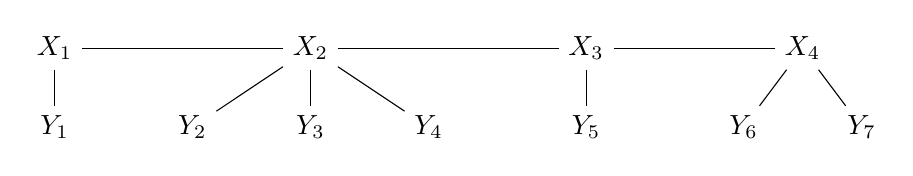
\begin{tikzpicture}%[scale=.8]
			\node[]  at (-0.25,0)  (w)  {$X_1$};
			\node[]  at (3,0) 		 (k)   {$X_2$};
			\node[]  at (6.5,0) 	(h)   {$X_3$};
			\node[]  at (9.25,0)   (l)    {$X_4$};
			\draw[] (w) -- (k);
			\draw[] (k) -- (h);
			\draw[] (h) -- (l);
			\node[]  at (-0.25,-1)(f1) {$Y_1$};
			\node[]  at (1.5,-1) 	 (f2) {$Y_2$};
			\node[]  at (3,-1) 	 (f3) {$Y_3$};
			\node[]  at (4.5,-1) 	(f4) {$Y_4$};
			\node[]  at (6.5,-1)	(f5) {$Y_5$};
			\node[]  at (8.5,-1)   (f6) {$Y_6$};
			\node[]  at (10,-1)  	(f7)  {$Y_7$};
			\draw[] (w) -- (f1);
			\draw[] (k) -- (f2);
			\draw[] (k) -- (f3);
			\draw[] (k) -- (f4);
			\draw[] (h) -- (f5);
			\draw[] (l) -- (f6);
			\draw[] (l) -- (f7);
		\end{tikzpicture}
		\caption{A directed graph for CAT\label{fig:fourskills}.}
	\end{figure}
	\vspace{-5mm}
	
	Teachers report their knowledge about the unconditional states of $X_1$ and the 
	conditional states of $X_i$ given $X_{i-1}$, for $i=2,3,4$, as qualitative judgments (top 
	of Tab.~\ref{tb:CPTs}). 
	To simplify the elicitation, the probabilities $P(X_i|X_{i-1})$ are given the same verbal 
	judgment for all $i=2,3,4$. A more detailed model could provide more accurate 
	evaluations but it would be very hard for the domain expert to elicit it in a reliable way. 
	Also, questions are divided by the teachers in three groups, corresponding to different 
	difficulty levels. Questions in the same group are quantified in the same way, 
	irrespective of their background skill, giving the judgments reported in the bottom part 
	of Tab.~\ref{tb:CPTs}. 
	
	{\small \begin{table*}[htp!] 
			\renewcommand{\arraystretch}{1.2}
			\centering
			{%\footnotesize
				\begin{tabular}{@{}lc@{}}
					\toprule
					$X_1$&$P(X_1)$\\
					\midrule
					A1&\emph{improbable}\\
					A2&\emph{uncertain}\\
					B1&\emph{uncertain}\\
					B2&\emph{improbable}\\
					\bottomrule
				\end{tabular}
				\quad
				\begin{tabular}{@{}lcccc@{}}
					\toprule	
					$P(X_i|X_{i-1})$&\phantom{.}$X_{i-1}=\mathrm{A1}$\phantom{.}&\phantom{.}$X_{i-1}=\mathrm{A2}$\phantom{.}&\phantom{.}$X_{i-1}=\mathrm{B1}$\phantom{.}&\phantom{.}$X_{i-1}=\mathrm{B2}$\phantom{.}\\
					\midrule
					$X_i$=A1&\emph{fifty-fifty}&\emph{uncertain}&\emph{improbable}&\emph{impossible}\\
					$X_i$=A2&\emph{uncertain}&\emph{fifty-fifty}&\emph{uncertain}&\emph{improbable}\\
					$X_i$=B1&\emph{improbable}&\emph{uncertain}&\emph{fifty-fifty}&\emph{uncertain}\\
					$X_i$=B2&\emph{impossible}&\emph{improbable}&\emph{uncertain}&\emph{fifty-fifty}\\
					\bottomrule
			\end{tabular}}
			\vskip 2mm
			\begin{tabular}{@{}lcccc@{}}\toprule
				$P(Y=T|X)$\phantom{aa}&\phantom{a}$X=\mathrm{A1}$\phantom{a}&\phantom{a}$X=\mathrm{A2}$\phantom{a}&\phantom{a}$X=\mathrm{B1}$\phantom{a}&\phantom{a}$X=\mathrm{B2}$\phantom{a}\\
				\midrule
				Easy&\emph{uncertain}&\emph{fifty-fifty}&\emph{expected}&\emph{probable}\\
				Medium&\emph{improbable}&\emph{uncertain}&\emph{fifty-fifty}& 
				\emph{expected}\\
				Difficult&\emph{impossible}&\emph{improbable}&\emph{uncertain}& 
				\emph{fifty-fifty}\\
				\bottomrule
			\end{tabular}
			\vskip 2mm
			\caption{Expert judgements.}\label{tb:CPTs}
	\end{table*}}
	%\vspace{-10mm}
	For the CN, those judgements are translated in interval constraints for the 
	corresponding events on the basis of the verbal-numerical scale in Tab.~\ref{tb:labels}. 
	Different probability intervals are considered for skills and questions as they refer to 
	events of different type. For instance, when the expert considers ``\emph{impossible}'' 
	for an A1 level student to know the answer to a difficult question, the student is 
	assigned a probability between .175 and .2 of answering correctly, as the questions 
	offer only four choices plus the option of giving no answer. 
	Notice that, by doing so, we are not anymore assuming that all questions in the same 
	difficulty group share exactly the same conditional PMFs (as done by the BN model), as 
	PMFs of different questions can vary independently in the given intervals. This seems a 
	more sensible assumption than that of the precise model.
	For the BN, the PMFs corresponding to the centers of mass of the CSs defining the CN 
	are used. Numerical inferences in the BN are consequently included in the intervals 
	computed with the CN.
	
	{\small
		\begin{table*}[htp!] 
			\renewcommand{\arraystretch}{1.2}
			\centering
			\begin{tabular}{@{}lcccccc@{}}
				\toprule
				Judgement&\emph{impossible}&\emph{improbable}&\emph{uncertain}&\emph{fifty-fifty}&\emph{expected}&\emph{probable}\\
				\midrule
				Skills&$1$-$10\%$&$10$-$20\%$&$20$-$40\%$&$30$-$50\%$&-&-\\
				Questions&$17.5$-$20\%$&$22.5$-$25\%$&$30$-$35\%$&$60$-$65\%$&$75$-$80\%$&
				 $95$-$97.5\%$\\
				\bottomrule
			\end{tabular}
			\caption{A verbal-numerical scale for probability-intervals 
			elicitation.}\label{tb:labels}
	\end{table*}}
	
	\paragraph{Experimental results.} 
	%Acronyms BN-NA, CN-NA, BN-AD, CN-AD denote 
	BN and CN methods in their non-adaptive (NA) and adaptive (AD) versions are 
	considered. \emph{Accuracy}, i.e., the proportion of students to whom the test assigns 
	the same level of the current evaluation method, describes BN performances. This 
	measure cannot be used for the set-valued outputs of CN methods. In this case the 
	$u_{65}$ measure can provide a comparison with the accuracy 
	\cite{zaffalon2012evaluating}. If $\mathcal{L}$ is the set of levels assigned by the CN 
	on a skill and $L$ its cardinality, a \emph{discounted} accuracy gives $1/L$ if 
	$\mathcal{L}$ includes the true level and zero otherwise. The $u_{65}$ is a concave 
	reinforcement of this score based on risk-adverse arguments. Its underlying 
	assumption is that acknowledging the indecision between more levels has larger utility 
	than randomly choosing one of them (e.g., the teacher could set up further 
	assessments in the undecided cases). Tab.~\ref{tb:nonAdaptiveResults} shows the NA 
	comparison. In Fig.~\ref{fig:plots} (left), the BN-NA accuracy is separately evaluated on 
	the determinate (light bars) and indeterminate (dark bars) instances, i.e. those for 
	which, respectively, a single level or multiple levels are returned by the CN model. On 
	average, CN-NA returns single levels in $37.25\%$ of the cases and, if this is not the 
	case, an average of $2.36$ levels ($3.22$ with interval dominance) are returned. 
	
	\begin{table*}[htp!]
		\centering
		\begin{tabular}{@{}lccccc@{}}\toprule
			Algorithm&\phantom{aa}Average\phantom{aa}&\phantom{aaa}$X_1$\phantom{aaa}&\phantom{aaa}$X_2$\phantom{aaa}&
			 \phantom{aaa}$X_3$\phantom{aaa}&\phantom{aaa}$X_4$\phantom{aaa}\\
			\midrule
			BN-NA (acc)&$63.09\%$&$	67.56	\%$&$60.85\%$&${	75.84	
			\%}$&$48.10\%$\\
			CN-NA ($u_{65}$)& ${65.37\%}$&$67.71\%$&${66.67\%}$&$	
			70.33\%$&${56.76\%}$\\
			\bottomrule
		\end{tabular}
		\caption{Non-adaptive tests results.}\label{tb:nonAdaptiveResults}
	\end{table*}
	
	In the AD case we also track the average number of asked questions. Results are in 
	Fig.~\ref{fig:plots} (right). CN-AD (circles) is tested for different thresholds over the 
	entropy (labels of the markers) against a version of BN-AD based on the joint entropy 
	(triangles). Similar values are obtained by coping with marginal entropies. We also allow 
	the BN-AD method to return multiple levels by maximizing the expected $u_{65}$ utility 
	over any possible set of levels. This variant is called BN-AD' and the corresponding 
	$u_{65}$ measure is reported  (squares).
	
	\begin{figure}[htp!]
		\centering
		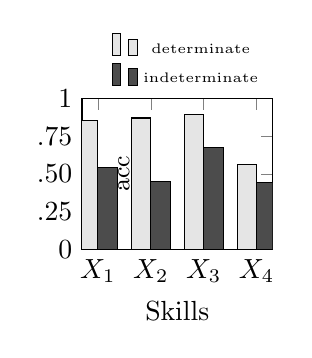
\begin{tikzpicture}
			\begin{axis}[width=4cm,height=3.5cm,ybar=0,bar width=7pt,ylabel={\small acc}, 
			xlabel={Skills},xtick=data,ytick={0,25,50,75,100},ymin=0,ymax=100,yticklabels={0,.25,.50,.75,1},symbolic
			 x coords={$X_1$,$X_2$,$X_3$,$X_4$}, y label style={at={(axis description 
			cs:0.3,.5)},anchor=south},xtick align=inside, legend 
			style={at={(1,1)},anchor=south east},legend style={draw=none}]
				\addplot[fill=black!10] coordinates 
				{($X_1$,85.42)($X_2$,87.06)($X_3$,89.51)($X_4$,56.34)}; 
				\addlegendentry{\tiny{determinate}} 
				\addplot[fill=black!70] coordinates 
				{($X_1$,54.51)($X_2$,45.13)($X_3$,67.72)($X_4$,44.26)};
				\addlegendentry{\tiny{indeterminate}}
			\end{axis}
		\end{tikzpicture}
		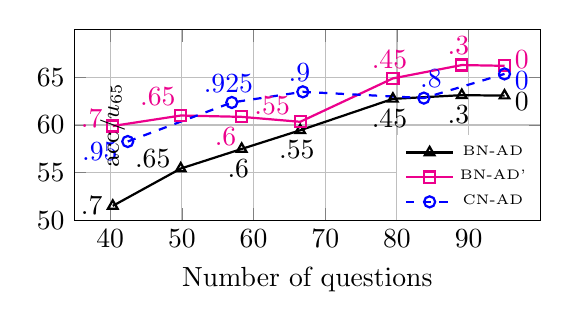
\begin{tikzpicture}
			\begin{axis}[width=7.5cm,height=4cm,ylabel={\small 
			acc/$u_{65}$},xlabel={Number of questions},xmin=35, xmax=100,ymin=50, 
			ymax=70, xtick={40,50,60,70,80,90}, ytick={50,55,60,65},legend 
			style={at={(1,0)},anchor=south east},ymajorgrids=true,xmajorgrids=true,  y label 
			style={at={(axis description cs:0.13,.5)},anchor=south},legend style={draw=none}]
				\addplot[black,thick,mark=triangle,mark options={fill=black}, visualization 
				depends on=\thisrow{alignment} \as \alignment, nodes near coords, point 
				meta=explicit symbolic,  every node near coord/.style={anchor=\alignment}] 
				table [meta index=2 ] {
					x y label alignment
					40.36	51.51 .7 0
					49.84	55.43 .65 -20
					58.34	57.49 .6 80
					66.50 59.45 .55 80
					79.43	62.75 .45 80
					89.04	63.14 .3 80
					95  63.09     0  160
				};
				\addlegendentry{\tiny{BN-AD}}
				\addplot[magenta,thick,mark=square,mark options={fill=black}, visualization 
				depends on=\thisrow{alignment} \as \alignment, nodes near coords, point 
				meta=explicit symbolic,  every node near coord/.style={anchor=\alignment}] 
				table [meta index=2 ] {
					x y label alignment
					40.36	59.9 .7 -20
					49.84	61.00 .65 -40
					58.34	60.86 .6 50
					66.50 60.34 .55 -30
					79.43	64.90 .45 -80
					89.04	66.3 .3 -80
					95  66.22     0  -160
				};
				\addlegendentry{\tiny{BN-AD'}}
				\addplot[dashed,blue,thick,mark=o,mark options={solid,fill=white},
				visualization depends on=\thisrow{alignment} \as \alignment,
				nodes near coords, % Place nodes near each coordinate
				point meta=explicit symbolic, % The meta data used in the nodes is not 
				%explicitly provided and not numeric
				every node near coord/.style={anchor=\alignment} ] table [meta index=2 ] {
					x       y   label  alignment
					42.45 58.27  .95   20
					56.96 62.37  .925   -80
					66.87 63.49   .9   -80
					83.75 62.83  .8    -110
					95   65.37   0  160
				};
				\addlegendentry{\tiny{CN-AD}}
			\end{axis}
		\end{tikzpicture}
		\caption{Non-adaptive (left) and adaptive (right) tests performance.}\label{fig:plots}
	\end{figure}
	
	
	As a comment, CNs seem to identify hard-to-evaluate students as those for which 
	multiple levels are provided. In fact, the agreement between the BN and the traditional 
	tests is larger when the CN test is determinate. As a consequence, the CN $u_{65}$ 
	measure is, on average, larger than the BN accuracy. 
	A limitation of the CN test is the large fraction of indeterminate evaluations. One can 
	interpret this result as a lack of robustness of the BN model, as even small variations in 
	the model specifications can result in different decisions. Results also show that, both 
	BN-AD and CN-AD approaches reduce the number of questions asked without 
	significantly affecting the accuracy. BN-AD performances are improved by the ``credal'' 
	variant BN-AD'. The results becomes very similar to those of the CN-AD. Yet, the latter 
	method appears to be a more principled and suitable approach for a direct modeling of 
	qualitative expert knowledge. 
	
	%does not require any, potentially questionable, imputation of the probabilistic ranges 
	%provided by the experts.
	
	%Yet, we regard theof BN-AD, we regard the CN approach as more principled and 
	%suitable for a direct modeling of qualitative expert knowledge.
	
	%uch a difference disappear if the credal-like variant BN-AD' is considered.
	%However, the CN-AD procedure appears to be more effective, as the $u_{65}$ 
	%accuracy measure decreases more slowly than the accuracies of BN-AD procedures.  
	%Finally,comparing the two BN-AD approaches, one can see that the use of the local 
	%instead of the joint entropy does not compromise the effectiveness of the adaptive 
	%approach. 
	
	
	
	%Different decision criteria for the assignment of the skill level, e.g., maximality or 
	%e-admissibility, should be considered.
	%As a consequence, although BNs achieve better performance when considering the 
	%discounted accuracy, CN tests should be preferred whenever the utility is better 
	%described by the U65 or U80 measures, that is, whenever being undecided between 
	%more level should be preferred than assigning one of them at random. 
	%As the true level of the students is unknown, this measure should be regarded as the 
	%agreement between to different evaluation strategies. 
	%\begin{mdframed}[hidealllines=true,backgroundcolor=blue!20]
	%\paragraph{Experimental results.} 
	%Tab.~\ref{tab:nonadaptive} shows in the non-adaptive case the relative agreement 
	%between the traditional evaluation method (TEM) and the two BN-based models (IBN 
	%and TBN), computed as the proportion of students to which the tests under 
	%comparison assign the same level, averaged over 10 runs of cross-validation. On 
	%average 15\% of the students are assigned to a different level with respect to the 
	%traditional method (although the difference is never more than one level). The reason 
	%is 
	%that the BN models account for the difficulty of the questions. E.g., a student with 
	%only 
	%70\% of correct answers could be assigned the level B2 if he/she has answered 
	%correctly a large number of difficult questions which a student of lower level could 
	%not 
	%have guessed just by chance. 
	%\end{mdframed}
	%
	%\begin{table}[htp!]
	%%\renewcommand{\arraystretch}{1.1}
	%\centering
	%\begin{tabular}{@{}p{2.5cm}p{1.2cm}p{1.2cm}p{1.2cm}p{1.2cm}p{1.2cm}@{}}\toprule
	%Algorithm&\multicolumn{1}{l}{W\"ort.}&\multicolumn{1}{l}{Komm.}&\multicolumn{1}{l}{H\"oren}&\multicolumn{1}{l}{Lesen}&\multicolumn{1}{l}{Overall}\\
	% 
	%\midrule
	%TEM vs IBN&.80 &.87 &.89 &.85 &.85 \\
	%TEM vs TBN&.79 &.87 &.88 &.83 &.84 \\
	%IBN vs TBN&.98 &.95 &.94 &.92 &.95 \\
	%\bottomrule
	%\end{tabular}
	%\caption{Relative agreement between models}\label{tab:nonadaptive}
	%\vspace{-0.cm}
	%\end{table}
	%\begin{table}[htp!]
	%%\renewcommand{\arraystretch}{1.1}
	%\centering
	%\begin{tabular}{@{}p{2.5cm}p{1.2cm}p{1.2cm}p{1.2cm}p{1.2cm}p{1.2cm}@{}}\toprule
	%Algorithm&\multicolumn{1}{l}{W\"ort.}&\multicolumn{1}{l}{Komm.}&\multicolumn{1}{l}{H\"oren}&\multicolumn{1}{l}{Lesen}&\multicolumn{1}{l}{Overall}\\
	% 
	%\midrule
	%TEM& .28 &	.82 &	.88 &	.79 &	.84 \\
	%IBN& .71 &	.89 &	.83 &	.87 &	.90 \\
	%TBN& .79 &	.91 &	.87 &	.89 &	.92 \\
	%\bottomrule
	%\end{tabular}
	%\caption{Split-half reliability}
	%\label{tab:halfsplit}
	%\vspace{-0.8cm}
	%\end{table}
	%\begin{mdframed}[hidealllines=true,backgroundcolor=blue!20]
	%In this view, we believe that our approach provides more reliable evaluations than the 
	%traditional one. Tab.~\ref{tab:halfsplit} shows the internal consistency of the three 
	%tests evaluated using the split-half methodology: the questions are randomly divided 
	%into two subset of equal size; the two half-tests thus obtained are used to generate 
	%two independent evaluations of the students; the correlation coefficient between the 
	%outputs of the two half-tests adjusted with the Spearman-Brown correction is 
	%retained 
	%as a measure of the test reliability. Results show that the reliability of both Bayesian 
	%approaches (IBN and TBN) is larger than that of the traditional method. TBN has the 
	%highest reliability, as it considers the correlation between different skills and thus all 
	%answers contribute to the determination of the level of a skill, even those referring to 
	%different skills. 
	%Concerning the adaptive case, we have considered different thresholds for the 
	%entropy. The left plot in Fig.~\ref{fig:agreement} shows the relative agreement of the 
	%adaptive tests using IBN and TBN with the non-adaptive TBN, whereas the right plot 
	%shows the average number of questions asked to the students. Both models show a 
	%strong reduction in the number of questions as the threshold on the entropy 
	%increases. 
	%For instance, using the TBN model, the number of questions reduces of about 70\% 
	%passing from the non-adaptive test to an adaptive test with entropy threshold 
	%$\tilde{H}=0.5$. Yet, the test still provides the same evaluations as the non-adaptive 
	%one in more than 70\% of the cases. Such an accuracy loss might be problematic. 
	%However, even decreasing the entropy threshold to $\tilde{H}=0.19$, we can still save 
	%20 question on average (to a maximum of 65 questions in the best case) at the price 
	%of 
	%a reduction of only 3\% in the accuracy. This shows that a significant number of 
	%questions provides very little information about the student level of knowledge. Our 
	%adaptive approach makes it possible to avoid wasting students' time asking 
	%uninformative questions. 
	%\end{mdframed}
	%\begin{figure}[htp!]
	%\centering
	%\begin{tikzpicture}
	%\begin{axis}[title={Agreement},width=6cm, height=4cm,xlabel={Entropy Threshold 
	%$\tilde{H}$},xmin=0, xmax=0.5, ymin=0.7, ymax=1, xtick={0,.1,.2,.3,.4,.5}, 
	%ytick={.7,.8,.9,1}, legend pos=north east, ymajorgrids=true, xmajorgrids=true]
	%\addplot[color=black,mark=square] coordinates { (0.0625,0.99833) (0.125,0.99217) 
	%(0.1875,0.9685) (0.25,0.89583) (0.375,0.75183) (0.5,0.74517)};    
	%\addlegendentry{TBN}
	%\addplot[color=black!60,mark=star] coordinates { 
	%(0.0625,0.94733)(0.125,0.946000)(0.1875,0.943333)(0.25,0.8965000)(0.375,0.744000)(0.5,0.724666)};
	%\addlegendentry{IBN}
	%\end{axis}
	%\end{tikzpicture}
	%\begin{tikzpicture}
	%\begin{axis}[ title={Number of questions},width=6cm, height=4cm, xlabel={Entropy 
	%Threshold $\tilde{H}$}, xmin=0, xmax=0.5, ymin=0, ymax=100, xtick={0,.1,.2,.3,.4,.5}, 
	%ytick={0,20,40,60,80,100}, legend pos=north east, ymajorgrids=true, 
	%xmajorgrids=true]
	%\addplot[color=black!60,mark=star] coordinates { (0.0625,89.741) (0.125,87.229) 
	%(0.1875,81.309) (0.25,66.745) (0.375,32.5) (0.5,29.001)};    
	%\addlegendentry{IBN}
	%\addplot[color=black,mark=square] coordinates { (0.0625,88.553) (0.125,83.476) 
	%(0.1875,75.071) (0.25,58.484) (0.375,30.722) (0.5,29)};
	%\addlegendentry{TBN}
	%\end{axis}
	%\end{tikzpicture}
	%\caption{Agreement between the adaptive methods and the non-adaptive TBN (left) 
	%and average number of questions asked by the adaptive methods 
	%(right)}\label{fig:agreement}
	%\vspace{-.8cm}
	%\end{figure}
	%As providing precise values for these probabilities can be very hard even for expert 
	%teachers, the subjective opinion about the likelihood of an event was described by 
	%using the verbal-numerical probability scales in Table \ref{tb:labels}. 
	%The question and skill CPTs are given in tables \ref{tb:questionCPTs} and 
	%\ref{tb:skillCPTs}.
	%make the model specification complete, the CPTs of the skills, i.e., $\{ 
	%P(X_i|\mathrm{\Pi_{X_i}})\}_{i=1}^4$, and those of the questions, i.e., $\{ 
	%P(Y_j|B_{Y_j})\}_{j=1}^{95}$ should be quantified.
	%In previous work \cite{mangili2016a}, these parameters have been learned from the 
	%available data. Results have shown that the resulting model can achieve larger internal 
	%consistency than the traditional evaluation method in assessing the student level. 
	%Given this result, a data-driven approach is used here to provide \emph{ground truth} 
	%evaluations for each student. This approach, hereafter referred to as EM-BN, uses 
	%expectation maximization (EM) to learn the CPTs of the BN model in  figure 
	%\ref{fig:fourskills} and infer the students level in the four skills. 
	%The focus of the paper, however, is to provide an approach to adaptive testing 
	%entirely based on expert elicitation. Therefore, 
	%As we are interested in adaptive testing entirely based on expert elicitation, teachers 
	%have been asked to elicit all CPTs in the model. 
	%Following \cite{zaffalon2012evaluating}, the $u_{65}$ descriptors slightly increases 
	%the discounted accuracy contribution (i.e., $1/L$ is the set of labels includes the 
	%correct one and zero otherwise) with a convex xxx. Note that this descriptors is 
	%knows. 
	%The above-described model has been used to evaluate the skills of the 451 students 
	%in the dataset. 
	%As a ground truth we take the result based on the percentage of correct answers.
	%Then, we have compared the effectiveness of the BN and CN-based adaptive 
	%approaches.
	%?? traditional method, come nel paper ITS, EM?? \todo{scegliere ground truth}. 
	% we adopt the following performance descriptors:
	%\begin{itemize}
	%\item discounted accuracy (disA), i.e., the average value of 
	%$\frac{I_{\mathcal{L}}(l)}{L}$, where $I$ is the indicator function and $l$ the true level. 
	%This can be regarded as the most unfavorable way (among the reasonable ones) to 
	%evaluate
	%credal classifiers;
	%\item set accuracy (setAcc), i.e., the average value of $I_{\mathcal{L}(l)}$. This can be 
	%regarded as the performance measure most favorable to a credal classifier;
	%\item the utility-discounted accuracy U65 and U80 \cite{zaffalon2012evaluating}, i.e., 
	%the average value of a concave function $u\bigl(\frac{I_{\mathcal{L}}(l)}{L}\bigr)$ of 
	%the 
	%discounted utility. This measure assumes that being undecided between $k$ levels is 
	%better than choosing the correct level with probability $1/k$. This measure accounts 
	%for 
	%risk aversion, which increases with $u(0.5)$. We have $u(0.5)=0.65$ and 
	%$u(0.5)=0.8$ 
	%for, respectively the U65 and the U80 measures; \footnote{Notice that with 
	%$u(0.5)=0.5$ we obtain the discounted accuracy measure.}
	%\item the average number of times the credal test is determinate, that is, it returns a 
	%single level (DET);
	%\item the accuracy of the Bayesian test when the credal test is determinate (detA) and 
	%when it is indeterminate (indA). These indicators can show the capability of the credal 
	%test to identify the students which are more difficult to evaluate;
	%\item the average cardinality of $\mathcal{L}$ (Csize).
	%\end{itemize}
	
	
	% ---- Bibliography ----
	%
	% BibTeX users should specify bibliography style 'splncs04'.
	% References will then be sorted and formatted in the correct style.
	%
	% \bibliography{mybibliography}
	%
\bibliographystyle{splncs04}
\bibliography{biblio}
\end{document}
